\ylDisplay{Läätsed} % Ülesande nimi
{Tanel Kiis} % Autor
{lõppvoor} % Voor
{2013} % Aasta
{G 1} % Ülesande nr.
{3} % Raskustase
{
% Teema: Geomeetriline-optika
\ifStatement
Jukul on suur hulk nõgusläätsi, mille fookuskauguste leidmiseks ta konstrueeris lihtsa
süsteemi. Ta suunas optilise peateljega paralleelse
laserikiire läbimõõduga $2R$ tuntud fookuskaugusega
$f_1$ koondava läätse keskpunkti, pärast mida koondus laserkiir ekraanil ühte punkti. Kui nüüd panna
fookuskaugusega $f_2$ nõguslääts võrdsele kaugusele koondavast läätsest ja
ekraanist, on laserkiire läbimõõt ekraanil~$2r$. Leidke $f_2$ eeldusel, et~$2f_2 < f_1$.
\fi


\ifHint
Ülesande lahendamiseks tasub vaadelda kõige äärmist kiirt, mis kumerläätse siseneb, ning abijoontega määratleda, kuidas vastav kiir optilist süsteemi läbib. Seejärel saab ära kasutada sarnaseid kolmnurki.
\fi


\ifSolution
\begin{center}
	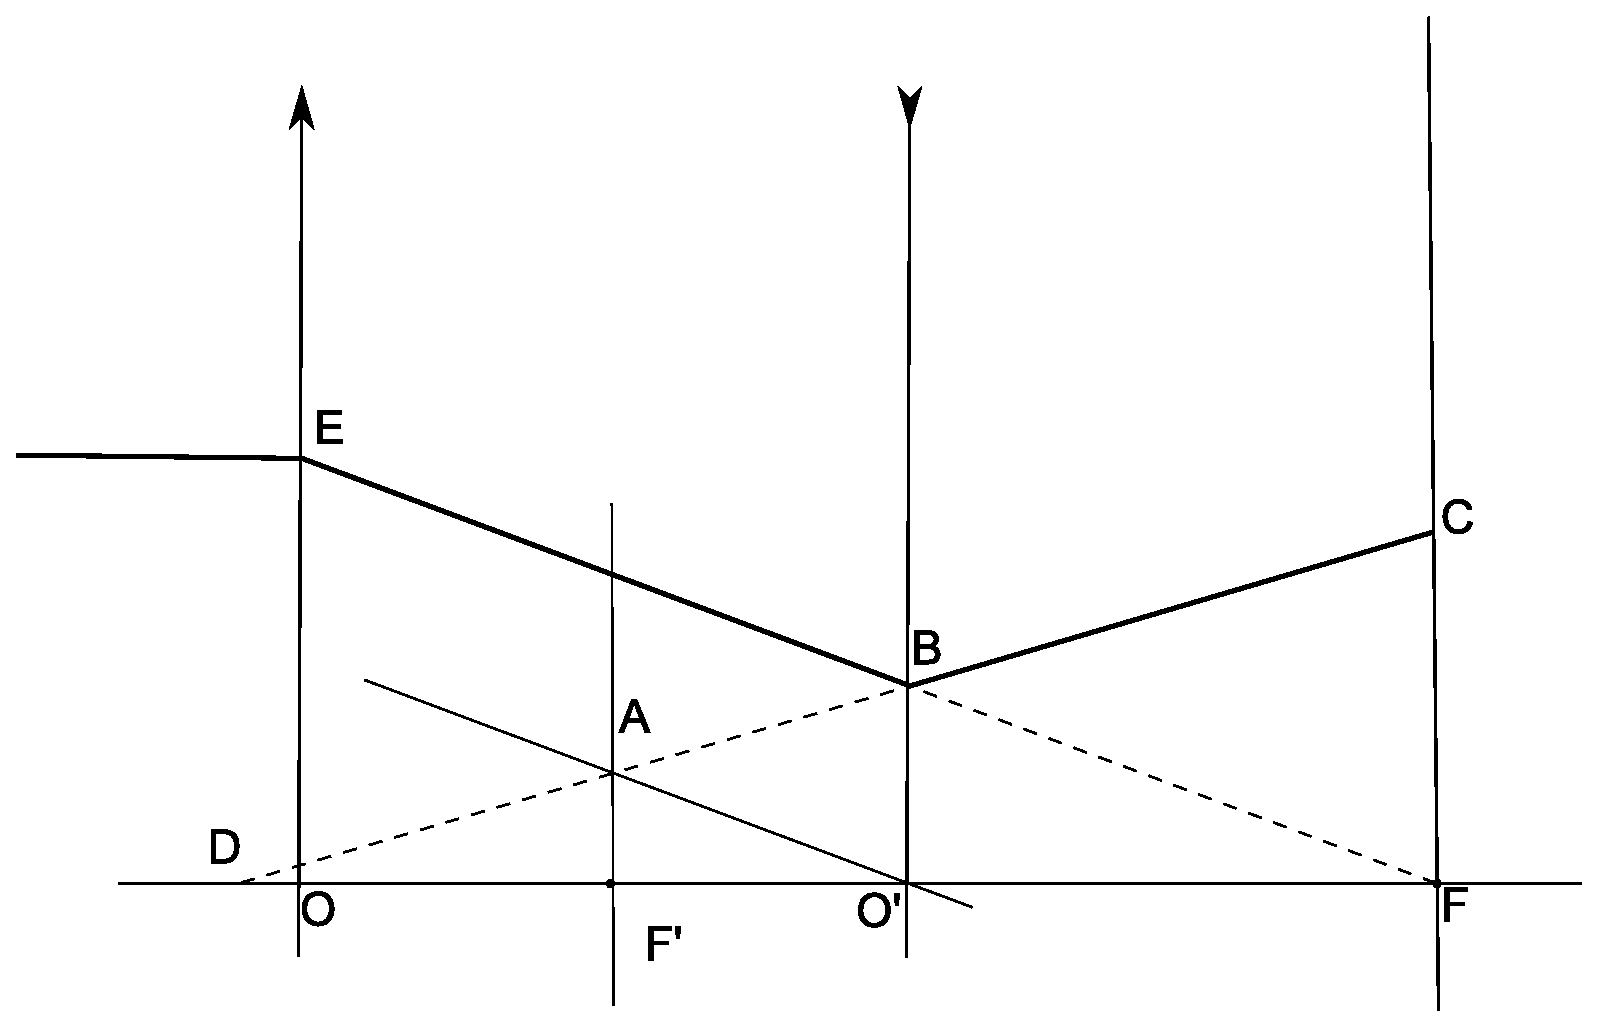
\includegraphics[width=0.8\textwidth]{2013-v3g-01-laats_lah2}\\
\end{center}
Kogu pilt on optilise peatelje suhtes sümeetriline, tänu sellele saame tegeleda ainult ühe poolega. Konstrueerime kiirte käigu, teades et kõigi nõgusläätse läbivate paraleelsete kiirte pikendused lõikuvad fokaaltasandil. 

Joonisel on mõned meid huvitavad sarnased kolmnurgad: $$\Delta AF'D \sim \Delta BO'D \sim \Delta CFD$$ ja $$\Delta EOF \sim \Delta AF'O' \sim \Delta BO'F.$$ Lisaks teame osade lõikude pikkusi: $|EO| = R$, $|OF| = f_1$, $|F'O'| = f_2$ ja $|CF| = r$.
Seda teades saab moodustada neljast võrrandist koosneva lineaarvõrrandisüsteemi.
\[ 
\begin{cases}
\frac{|EO|}{|OF|} = \frac{|AF'|}{F'O}\\
\frac{|EO|}{|OF|} = \frac{|BO'|}{O'F}\\
\frac{|AF'|}{|F'D|} = \frac{|CF|}{|FD|}\\
\frac{|AF'|}{|F'D|} = \frac{|BO'|}{|O'D|},\\
\end{cases}
\]
\[ 
\begin{cases}
\frac{R}{f_1} = \frac{|AF'|}{f_2}\\
\frac{R}{f_1} = \frac{|BO'|}{\frac{f_1}{2}}\\
\frac{|AF'|}{|O'D| - f_2} = \frac{r}{\frac{f_1}{2} + |O'D|}\\
\frac{|AF'|}{|O'D| - f_2} = \frac{|BO'|}{|O'D|}.\\
\end{cases}
\]

Pärast süsteemi lahendamist saame tulemuseks $f_2 = \frac{R}{4r}f_1$. 

\vspace{0.5\baselineskip}
\emph{Alternatiivne lahendus}\\

\begin{center}
	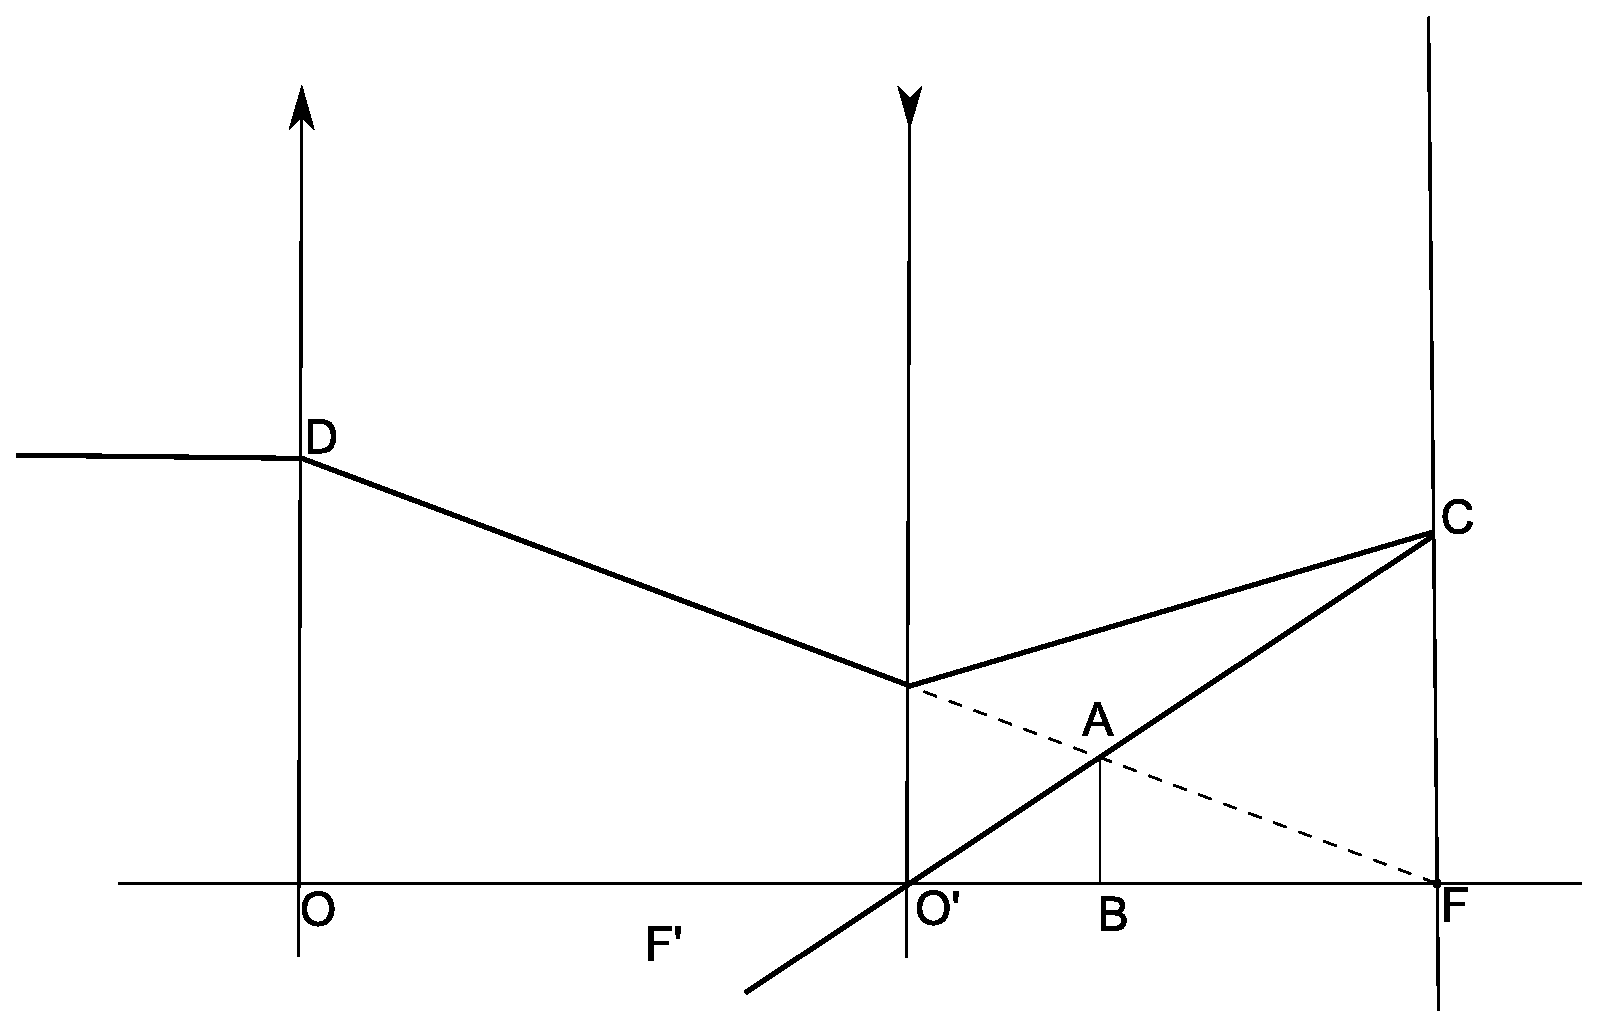
\includegraphics[width=0.9\textwidth]{2013-v3g-01-laats_lah3}\\
\end{center}

Selles lahenduses kasutame läätse valemit $-\frac{1}{f} = \frac{1}{a} - \frac{1}{k}$. $f$ ees on miinus, kuna tegemist on nõgusläätsega, ja $k$ ees on miinus, kuna tegemist on näiva kujutisega. Kasutades kiirte pööratavuse printsiipi vaatame hoopis olukorda, kus tekib objektist $CF$ näiv kujutis $AB$. Lisaks kasutame kolmnurkade sarnasust: $\Delta CFO' \sim \Delta ABO'$ ja $\Delta DOF \sim \Delta ABF$.

\[ 
\begin{cases}
\frac{|CF|}{|FO'|} = \frac{|AB|}{|BO'|}\\
\frac{|DO|}{|OF|} = \frac{|AB|}{|BF|}\\
-\frac{1}{f_2} = \frac{1}{|FO'|} - \frac{1}{|BO'|},\\
\end{cases}
\]
\[ 
\begin{cases}
\frac{r}{\frac{f_1}{2}} = \frac{|AB|}{|BO'|}\\
\frac{R}{f_1} = \frac{|AB|}{\frac{f_1}{2} - |BO'|}\\
-\frac{1}{f_2} = \frac{1}{\frac{f_1}{2}} - \frac{1}{|BO'|}.\\
\end{cases}
\]
Selle võrrandisüsteemi lahendamisel saame  $f_2 = \frac{R}{4r}f_1$.
\fi


\ifEngStatement
% Problem name: Lenses
Juku has a large number of concave lenses and to find their focal lengths he constructed a simple diagram. He directed a laser ray of diameter $2R$, parallel to the optical axis, to the center of a convex lens with a known focal length $f_1$, after that the ray is converged on one point on the screen. If a concave lens of focal length $f_2$ is now positioned at equal distance from the convex lens and the screen, then the diameter of the laser ray on the screen is $2r$. Find $f_2$ assuming that $2f_2 < f_1$.
\fi


\ifEngHint
To solve the problem you should observe the outermost ray that enters the convex lens and with auxiliary lines determine how the respective ray goes through the optical system. After that similar triangles can be used.
\fi


\ifEngSolution
\begin{center}
	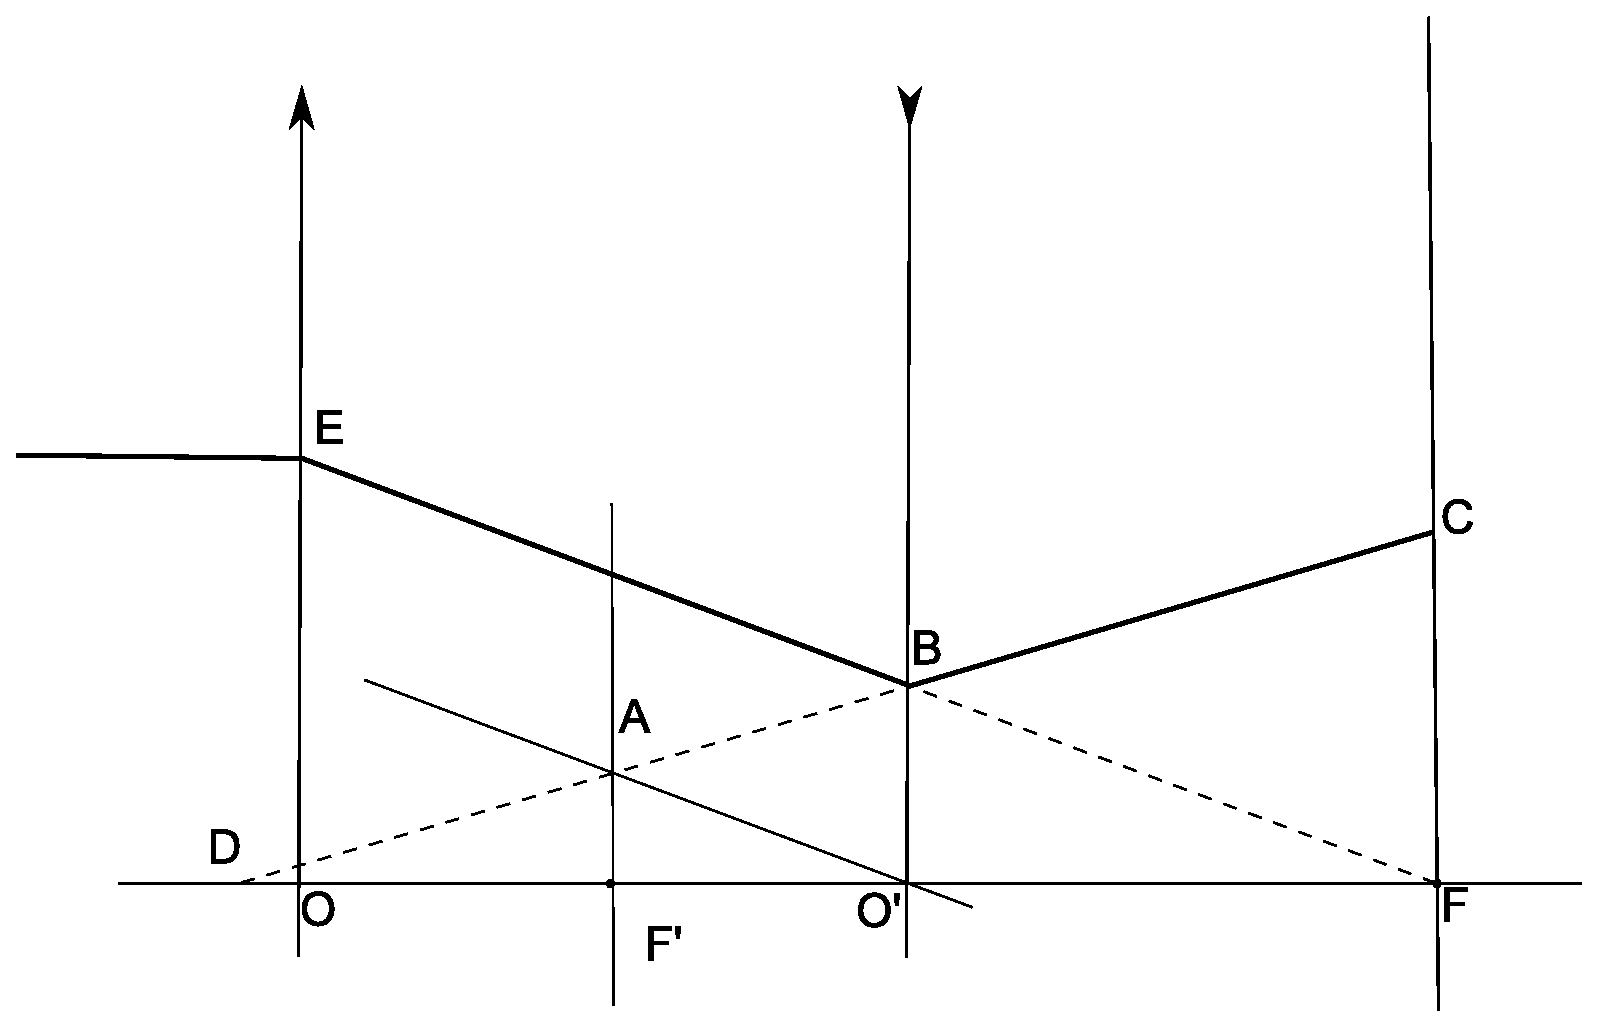
\includegraphics[width=0.8\textwidth]{2013-v3g-01-laats_lah2}\\
\end{center}
The whole picture is symmetrical with respect to the optical axis, thanks to this we can only study one side. We construct the path of the rays knowing that the extensions of all the parallel rays going through the concave lens intersect on focal plane.\\
In the figure there are some similar triangles of interest to us:
$$\Delta AF'D \sim \Delta BO'D \sim \Delta CFD$$ 
and 
$$\Delta EOF \sim \Delta AF'O' \sim \Delta BO'F.$$ 
In addition we know the lengths of some of the line segments: $|EO| = R$, $|OF| = f_1$, $|F'O'| = f_2$ and $|CF| = r$. Knowing this we can construct a system of linear equations consisting of four equations.
\[ 
\begin{cases}
\frac{|EO|}{|OF|} = \frac{|AF'|}{F'O}\\
\frac{|EO|}{|OF|} = \frac{|BO'|}{O'F}\\
\frac{|AF'|}{|F'D|} = \frac{|CF|}{|FD|}\\
\frac{|AF'|}{|F'D|} = \frac{|BO'|}{|O'D|},\\
\end{cases}
\] 
\[ 
\begin{cases}
\frac{R}{f_1} = \frac{|AF'|}{f_2}\\
\frac{R}{f_1} = \frac{|BO'|}{\frac{f_1}{2}}\\
\frac{|AF'|}{|O'D| - f_2} = \frac{r}{\frac{f_1}{2} + |O'D|}\\
\frac{|AF'|}{|O'D| - f_2} = \frac{|BO'|}{|O'D|}.\\
\end{cases}
\]
After solving the system we get the result $f_2 = \frac{R}{4r}f_1$.\\

\emph{Alternative solution}
\begin{center}
	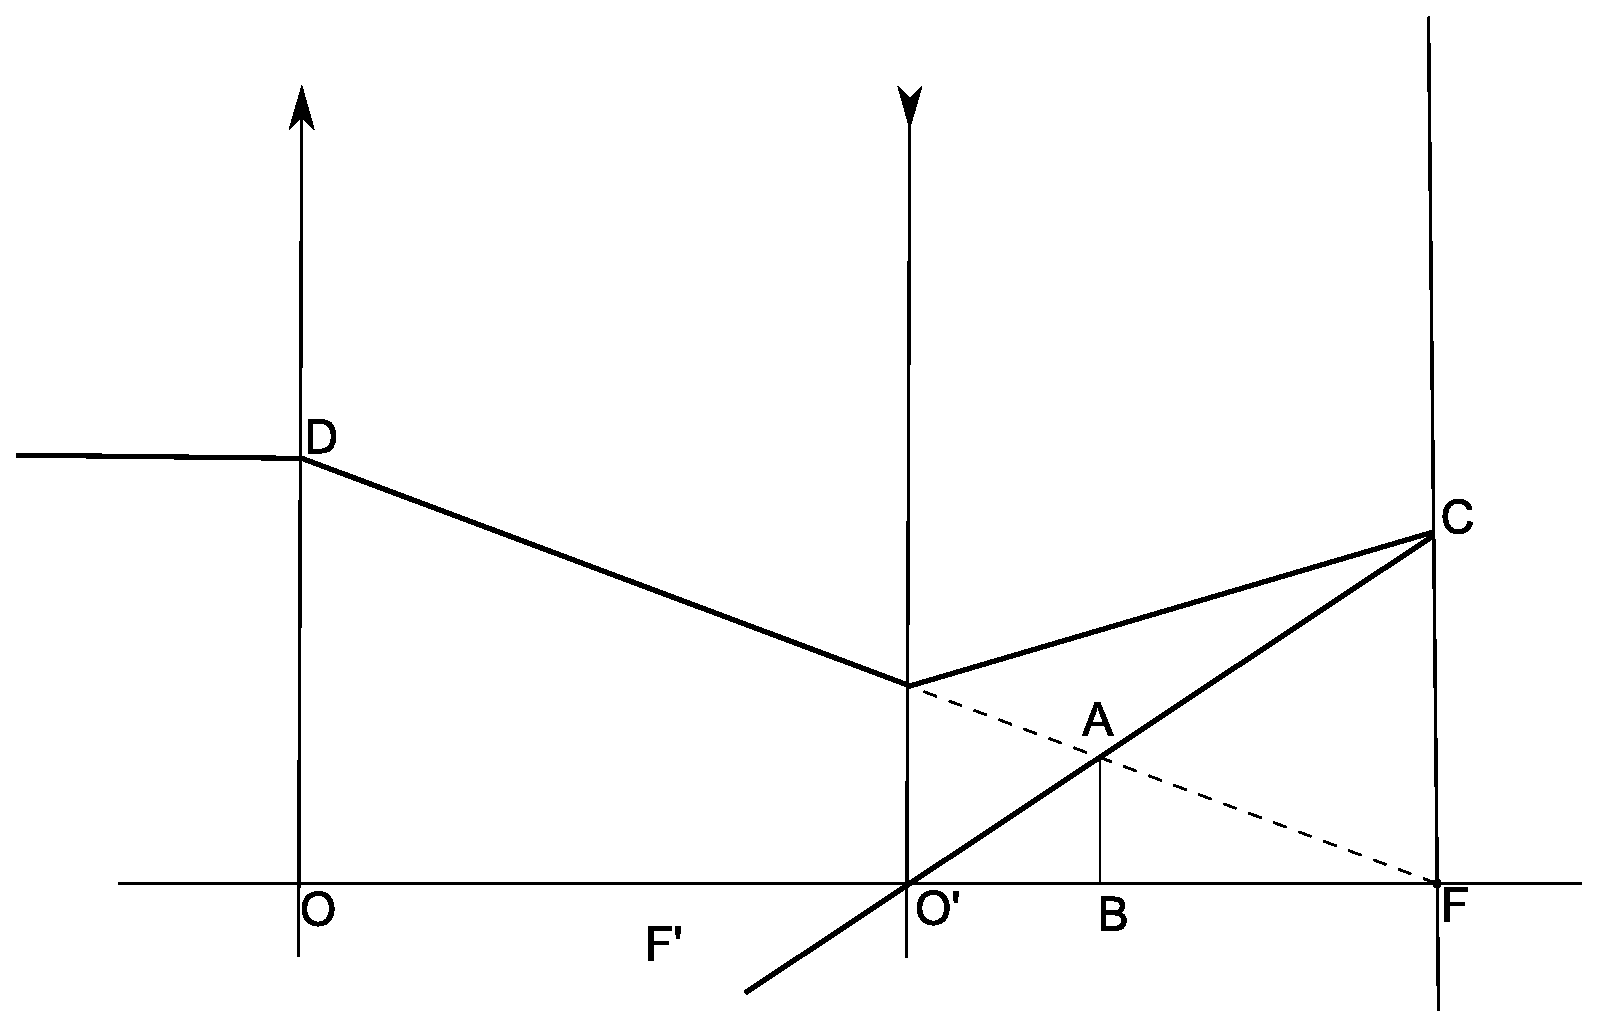
\includegraphics[width=0.9\textwidth]{2013-v3g-01-laats_lah3}\\
\end{center}
In this solution we use the thin lens formula $-\frac{1}{f} = \frac{1}{a} - \frac{1}{k}$. There is a minus in front of $f$ because we are dealing with a concave lens and a minus in front of $k$ because it is a virtual image. Using the principle of reversibility of light we instead study the situation where a virtual image $AB$ of object $CF$ appears. In addition we use similar triangles: $\Delta CFO' \sim \Delta ABO'$ and $\Delta DOF \sim \Delta ABF$.
\[ 
\begin{cases}
\frac{|CF|}{|FO'|} = \frac{|AB|}{|BO'|}\\
\frac{|DO|}{|OF|} = \frac{|AB|}{|BF|}\\
-\frac{1}{f_2} = \frac{1}{|FO'|} - \frac{1}{|BO'|},\\
\end{cases}
\]
\[ 
\begin{cases}
\frac{r}{\frac{f_1}{2}} = \frac{|AB|}{|BO'|}\\
\frac{R}{f_1} = \frac{|AB|}{\frac{f_1}{2} - |BO'|}\\
-\frac{1}{f_2} = \frac{1}{\frac{f_1}{2}} - \frac{1}{|BO'|}.\\
\end{cases}
\]
Solving this system of equations we get $f_2 = \frac{R}{4r}f_1$.
\fi
}